\documentclass{article}

\usepackage[polish]{babel}
\usepackage[T1]{fontenc}
\usepackage{geometry}
\usepackage{graphicx}

\geometry{margin=2.0cm}

\begin{document}

\begin{titlepage}
  \begin{center}
    % Nazwa uczelni / wydziału (opcjonalnie, warto dodać dla profesjonalnego wyglądu)
    {\large \textbf{Politechnika Wrocławska}} \\[0.3cm]
    {\normalsize Wydział Informatyki i Telekomunikacji} \\[2cm]

    % Nazwa laboratoriów
    {\Large \textbf{Sygnały i Obrazy Cyfrowe - Laboratorium}} \\[1.5cm]

    % Tytuł ćwiczenia w ramce lub z liniami ozdobnymi
    \rule{\textwidth}{0.4mm} \\[0.4cm]
    {\huge \bfseries Zastosowania splotu: rozpoznawanie tekstu 12.11.2026} \\[0.4cm]
    \rule{\textwidth}{0.4mm} \\[2.5cm]

    % Sekcja z autorami i prowadzącym
    \begin{minipage}{0.48\textwidth}
      \begin{flushleft}
        \textbf{Autor:} \\
        Michał Bernaś \\
        Nr indeksu: 290052 \\
        % Miejsce na termin laboratoriów
        Termin: Czwartek, 15:15
      \end{flushleft}
    \end{minipage}
    ~
    \begin{minipage}{0.48\textwidth}
      \begin{flushright}
        \textbf{Prowadzący:} \\
        dr hab. inż. Przemysław Śliwiński
      \end{flushright}
    \end{minipage}

    \vfill

    % Data / Miejsce
    {\large Wrocław, 2026}
  \end{center}
\end{titlepage}

\clearpage

\section{Cel ćwiczenia}
Celem ćwiczenia było zbadanie możliwości zastosowania splotu oraz korelacji wzajemnej w procesie automatycznego rozpoznawania tekstu na obrazach rastrowych. W ramach ćwiczenia zaimplementowano algorytm wykrywający i lokalizujący znaki na podstawie przygotowanych wzorców, a następnie odtwarzający tekst na ich podstawie. Porównano skuteczność obu metod oraz zbadano wpływ szumu Poissona na poprawność rozpoznawania. Dodatkowo zaproponowano alternatywne rozwiązanie, które mogłoby zwiększyć skuteczność rozpoznawania tekstu przy innych krojach czcionek lub piśmie odręcznym.

\section{Wstęp teoretyczny}
\subsection{Szum Poissona}
Szum Poissona, nazywany również szumem śrutowym, jest rodzajem zakłuceń występujących między innymi podczas rejestrowania obrazów za pomocą matryc światłoczułych. Wynika on z losowego charakteru procesu rejestracji fotonów. Liczba fotonów zarejestrowanych w określonym przedziale czasu może być opisana rozkładem Poissona: $$ P(X=k|\lambda) = \frac{\lambda^k e^{-\lambda}}{k!} $$ gdzie:
\begin{itemize}
  \item $X$ - liczba zarejestrowanych fotonów
  \item $k$ - konkretna liczba zarejestrowanych fotonów
  \item $\lambda$ - średnia liczba fotonów w danym przedziale czasu
\end{itemize}

Wartość parametru $\lambda$ wpływa na poziom zakłuceń obrazu. Im mniejsza średnia liczba rejestrowanych fotonów, tym większy względny wpływ szumu na uzyskany obraz.

\subsection{Splot i korelacja wzajemna}
Splot jest operacją matematyczną wykorzystywaną między innymi w cyfrowym przetwarzaniu sygnałów i obrazów. Polega na przesuwaniu odpowiedzi impulsowej filtra względem przetwarzanego sygnału i obliczaniu sumy iloczynów odpowiadających sobie próbek.

Dla sygnałów dyskretnych splot można zapisać jako: $$ (\lambda * f)(x_n) = \sum_{k = -\infty}^{+\infty} \lambda_k f(x_{n-k}) $$ gdzie $\lambda_k$ oznacza współczynniki filtra, natomiast $f(x_n)$ jest przetwarzanym sygnałem.

W przypadku obrazów operacja ta jest rozszerzana na dwa wymiary. Filtr przesuwany jest kolejno wzdłuż wierszy i kolumn obrazu, a dla każdej pozycji obliczana jest suma iloczynów jego współczynników i odpowiadającego im fragmentu obrazu.

Korelacja wzajemna jest operacją zbliżoną do splotu. Różnica polega na sposobie indeksowania próbek sygnału. Dla przypadku jednowymiarowego można ją zapisać jako: $$ (\lambda \star f)(x_n) = \sum_{k=-\infty}^{+\infty} \lambda_k f(x_{k+n}) $$

W praktyce oznacza to, że podczas obliczania splotu filtr jest odwracany względem obu osi, natomiast przy korelacji wzajemnej wykorzystywany jest w pierwotnej orientacji. Jeżeli filtr jest symetryczny, wyniki obu operacji mogą być identyczne.

\subsection{Wykorzystanie splotu i korelacji do rozpoznawania tekstu}
Splot i korelacja wzajemna mogą być wykorzystane do wykrywania określonych wzorców w obrazach. W przypadku rozpoznawania tekstu wzorcami są obrazy poszczególnych znaków, które pełnią funkcję filtrów.

Przesuwając filtr reprezentujący konkretny znak po obrazie wejściowym, można określić, w których miejscach występuje największe podobieństwo między wzorcem, a fragmentem obrazu. Wartości uzyskane w wyniku filtrowania pozwalają zlokalizować potencjalne wystąpienia znaków i przypisać im odpowiednie klasy.

Po wykryciu znaków konieczne jest również określenie ich kolejności na podstawie położenia na obrazie. Pozwala to odtworzyć pierwotny tekst w postaci ciągu znaków.

Skuteczność takiego podejścia zależy między innymi od jakości obrazu wejściowego, podobieństwa wzorców do rzeczywistych znaków oraz obecności zakłuceń. Szum może zmieniać wartości pikseli, przez co fragmenty obrazu stają się mniej podobne do przygotowanych wzorców, utrudniając prawidłową detekcję i rozpoznawanie znaków.

\section{Metoda realizacji i wykorzystane narzędzia}
W celu zrozumienia i zaprezentowania procesu rozpoznawania tekstu za pomocą splotu i korelacji wzajemnej przygotowano symulację w języku Python, wykorzystując biblioteki NumPy, Pillow, Matplotlib, SciPy oraz PyTorch.

Program generuje obraz zawierający tekst, a następnie nakłada na niego szum Poissona. Kolejnym etapem jest wyszukiwanie na obrazie najlepiej dopasowanych fragmentów za pomocą splotu lub korelacji wzajemnej, przy wykorzystaniu wcześniej przygotowanych wzorców poszczególnych znaków. Wykryte znaki są następnie porządkowane na podstawie ich położenia na obrazie, co pozwala odtworzyć tekst w postaci ciągu znaków. Na koniec obliczana jest skuteczność rozpoznawania poprzez porównanie odtworzonego tekstu z tekstem oryginalnym.

Dodatkowo program umożliwia alternatywne klasyfikowanie znaków z wykorzystaniem sieci neuronowej, która klasyfikuje wykryte fragmenty. Fragmenty, na których znajdują się litery wykrywane są za pomocą szukania jednolitych białych fragmentów, które są przekazywane sieci neuronowej w celu klasyfikacji, a sklasyfikowane znaki są przekazywane do funkcji, która składa z nich odtworzony tekst

Podczas przygotowywania programu korzystano również z narzędzi sztucznej inteligencji, które wspomagały proces implementacji oraz rozwiązywania napotkanych problemów.

\subsection{Sposób obliczania skuteczności rozpoznawania}
Skuteczność rozpoznawania tekstu określana jest poprzez porównanie tekstu odtworzonego przez algorytm z tekstem oryginalnym. Znaki znajdujące się na odpowiadających sobie pozycjach obu ciągów są porównywane ze sobą. W przypadku zgodności znak uznawany jest za poprawnie rozpoznany, natomiast w przypadku różnicy - za błędnie rozpoznany.

Skuteczność wyrażana jest procentowo jako stosunek liczby poprawnie rozpoznanych znaków do całkowitej liczby znaków w tekście oryginalnym.

Zastosowana metoda ma jednak pewne ograniczenia. Zakłada ona, że oba ciągi znaków zachowują zgodność pozycyjną. W przypadku pominięcia lub dodania znaku przez algorytm kolejne znaki mogą zostać porównane z niewłaściwymi odpowiednikami, co może prowadzić do zaniżenia uzyskanej skuteczności. Ponadto przy różnej długości ciągów funkcja porównująca znaki na odpowiadających sobie pozycjach nie uwzględnia automatycznie wszystkich dodatkowych znaków w dłuższym ciągu. Z tego względu ocena badanych algorytmów zależała również od czytelności odtworzonego tekstu, czyli czy człowiek czytając ten tekst jest w stanie łatwo zrozumieć sens oryginalnego tekstu.

\clearpage

\subsection{Fragment kodu symulacji}
\begin{verbatim}
  def fit_chars(image, filters, method):
  # Zbiór macierzy wynikowych splotu/korelacji przypisany do każdego znaku
  results = {}

  # Normalizacja obrazu do wartości od -1 do 1
  image = image / 127.5 - 1

  # Pętla iterująca po wszystkich filtrach
  for key, f in filters.items():
    # Normalizacja filtru do wartości od -1 do 1
    filter = f / 127.5 - 1

    # Jeżeli wykonywana jest operacja splotu, filtr jest obracany
    if method == "convolution":    
      filter = np.flip(filter, axis=(0, 1))

    # Pusta macież do której zostanie wpisany wynik splotu lub korelacji dla każdego piksela
    result = np.zeros((
      len(image) - len(filter) + 1,
      len(image[0]) - len(filter[0]) + 1
    ))

    # Wygenerowanie wszystkich możliwych fragmentów obrazu o wielkości filtra
    fragments = sliding_window_view(image, filter.shape)

    # Wykonanie splotu/korelacji każdego fragmentu obrazu z filtrem
    result = np.einsum("ijkl,kl->ij", fragments, filter)

    # Norma filtra
    filter_norm = np.sqrt(np.sum(filter ** 2))

    # Norma każdego fragmentu obrazu
    fragment_norm = np.sqrt(np.sum(fragments ** 2, axis=(2, 3)))

    # Normalizacja wyniku
    result = result / (fragment_norm * filter_norm + 1e-8)

    results[key] = result

  return results
\end{verbatim}

Zaprezentowany fragment kodu prezentuje funkcję odpowiedzialną za rozpoznawanie znaków za pomocą splotu lub korelacji wzajemnej. Funkcja przyjmuje jako argumenty obraz wejściowy, filtry przedstawiające pojedyncze litery oraz metodę z jakiej ma skorzystać (splot lub korelacja wzajemna). Zwraca słownik z macieżami wynków splotu lub korelacj dla przypisaną do każdego znaku.

\clearpage

\section{Przebieg ćwiczenia i uzyskane wyniki}
\begin{figure}[ht]
  \centering
  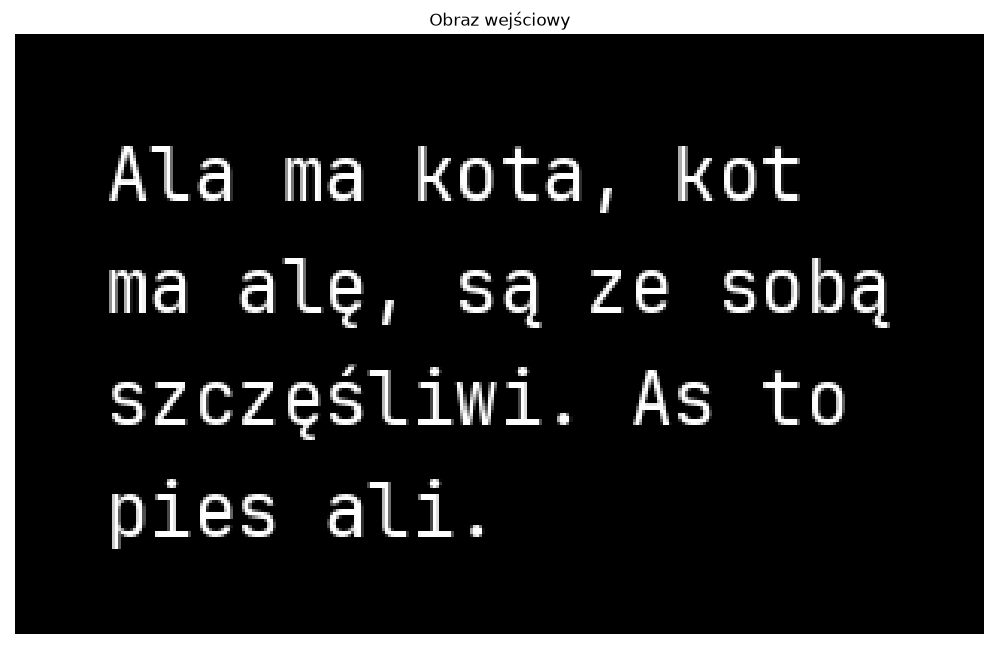
\includegraphics[width=0.7\linewidth]{Obrazy/ObrazWejściowy.png}
  \caption{Analizowany obraz wejściowy}
\end{figure}

\subsection{Rozpoznawanie tekstu za pomocą splotu}
\subsubsection{Brak szumu Poissona}

\begin{figure}[ht]
  \centering
  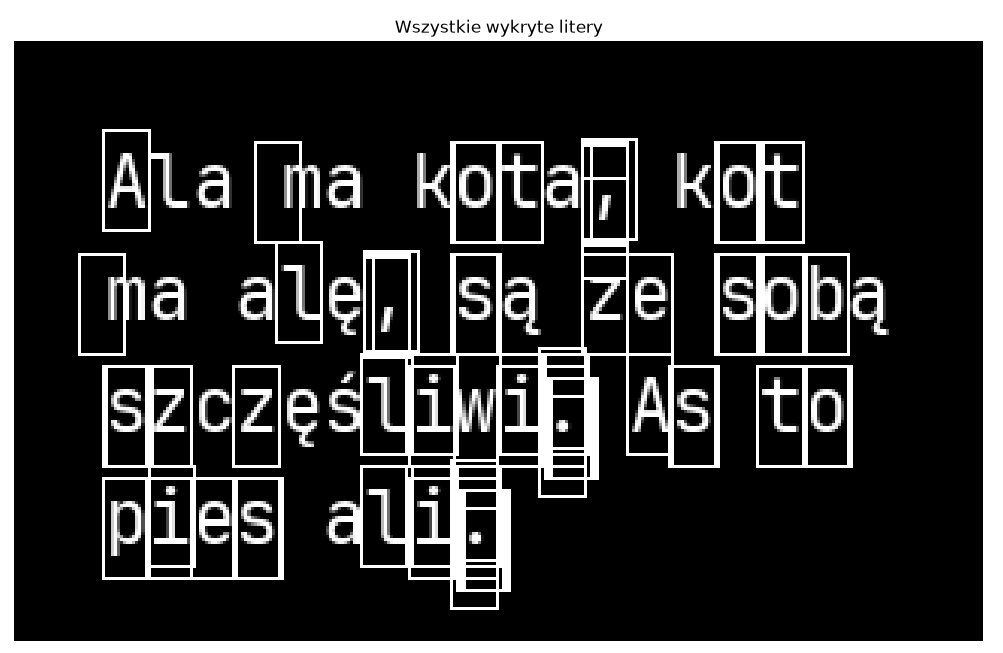
\includegraphics[width=0.7\linewidth]{Obrazy/Splot/WykryteZnaki.png}
  \caption{Wykryte znaki}
\end{figure}

Odtworzony tekst: V r oi ' oi r l ' s ze soq sz z lT T.~ Vs io dTes lT.~ \\
Skuteczność: 6\% \\
Ocena czytelności: Rozpoznany tekst nie przypomina tekstu na obrazie wejściowym. Nie można z niego wywnioskować jaka treść została napisana na obrazie.

\subsubsection{Szum Poissona dla $\lambda = 16$}

\begin{figure}[ht]
  \centering
  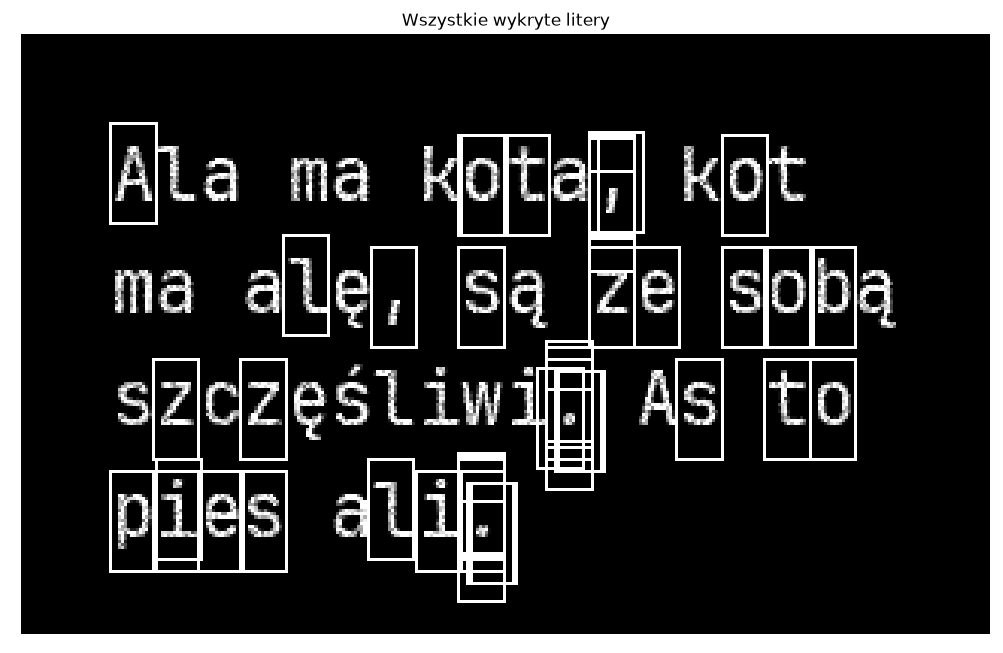
\includegraphics[width=\linewidth]{Obrazy/Splot/WykryteZnaki16.png}
  \caption{Wykryte znaki}
\end{figure}

Odtworzony tekst: V ci ' o l ' s ze soq z z .~ s io dTes lt.~ \\
Skuteczność: 6\% \\
Ocena czytelności: Rozpoznany tekst nie przypomina tekstu na obrazie wejściowym. Nie można z niego wywnioskować jaka treść została napisana na obrazie.

\clearpage

\subsubsection{Szum Poissona dla $\lambda = 4$}

\begin{figure}[ht]
  \centering
  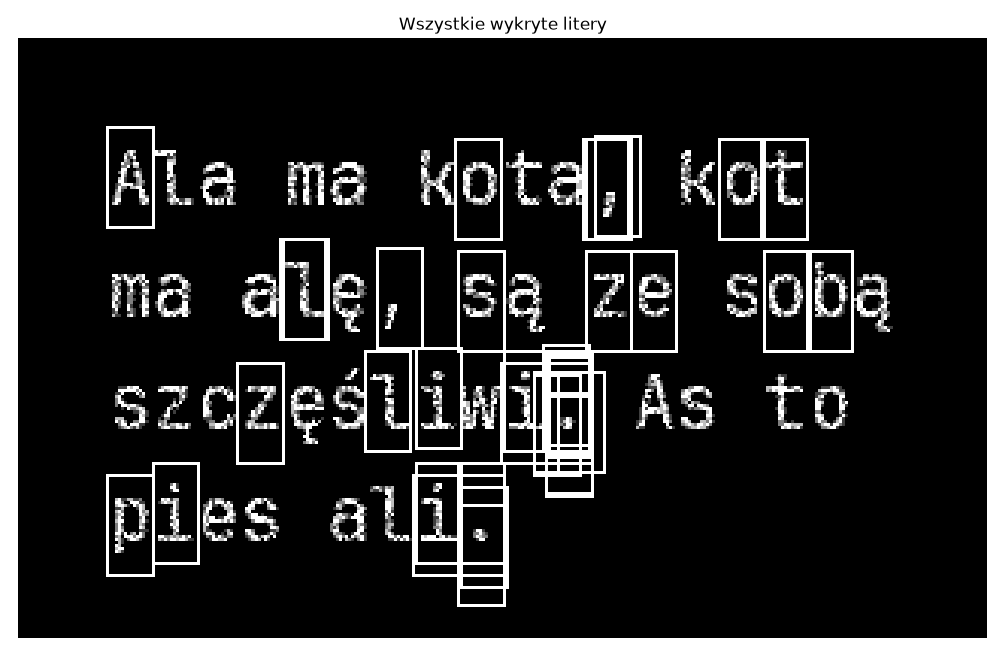
\includegraphics[width=\linewidth]{Obrazy/Splot/WykryteZnaki4.png}
  \caption{Wykryte znaki}
\end{figure}

Odtworzony tekst: V u " oi l " s `ze cq z l! T~.~ dT T. \\
Skuteczność: 3\% \\
Ocena czytelności: Rozpoznany tekst nie przypomina tekstu na obrazie wejściowym. Nie można z niego wywnioskować jaka treść została napisana na obrazie.

\clearpage

\subsubsection{Szum Poissona dla $\lambda = 1$}

\begin{figure}[ht]
  \centering
  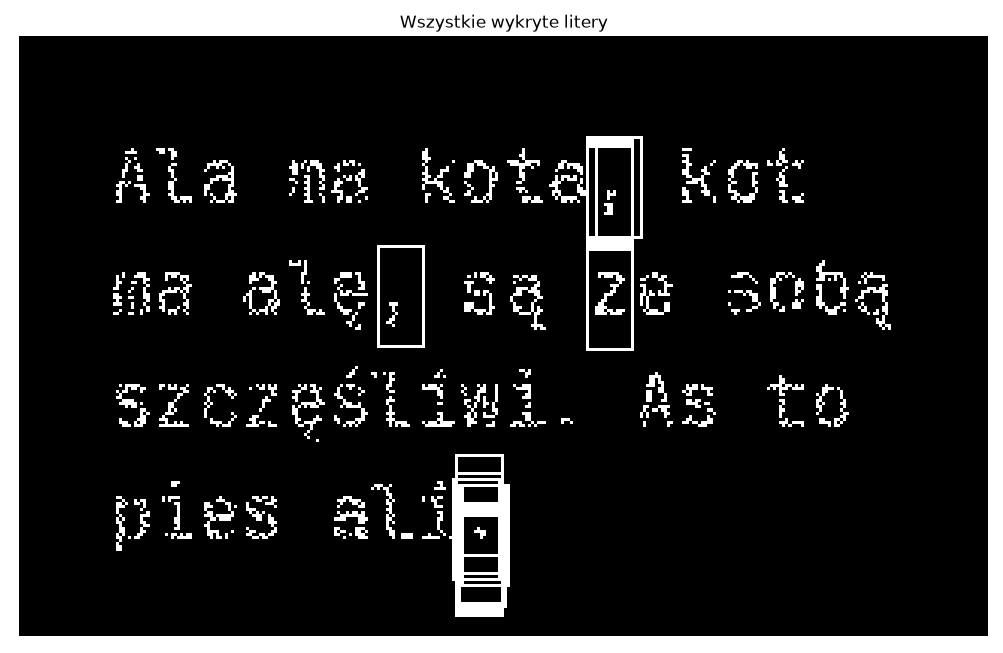
\includegraphics[width=\linewidth]{Obrazy/Splot/WykryteZnaki1.png}
  \caption{Wykryte znaki}
\end{figure}

Odtworzony tekst: ' " z ` \\
Skuteczność: 1\% \\
Ocena czytelności: Większość znaków nie została rozpoznana. Z odtworzonego tekstu nie można ustalić sensu oryginalnego tekstu.

\clearpage

\subsection{Rozpoznawanie tekstu za pomocą korelacji wzajemnej}
\subsubsection{Brak szumu Poissona}

\begin{figure}[ht]
  \centering
  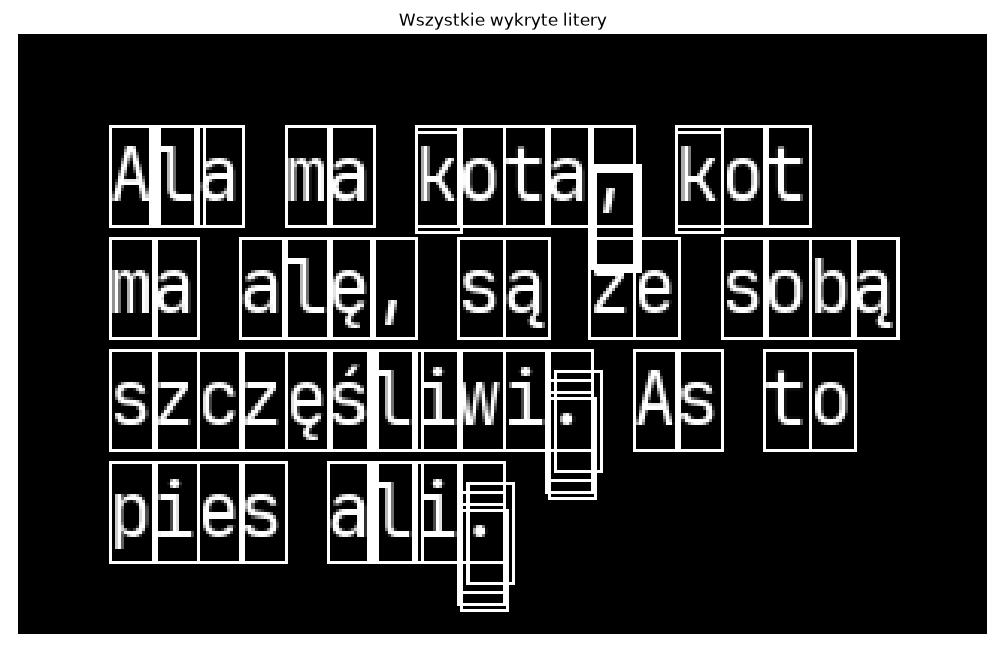
\includegraphics[width=\linewidth]{Obrazy/Korelacja/WykryteZnaki.png}
  \caption{Wykryte znaki}
\end{figure}

Odtworzony tekst: Ala ma kota, kot ma alę, są ze sobą szczęśliwi. As to pies ali. \\
Skuteczność: 100\% \\
Ocena czytelności: Odtworzony tekst jest identyczny z tekstu znajdującego się na obrazie wejściowym. Bez problemu można zrozumieć sens odtworzonego sensu.

\clearpage

\subsubsection{Szum Poissona dla $\lambda = 16$}

\begin{figure}[ht]
  \centering
  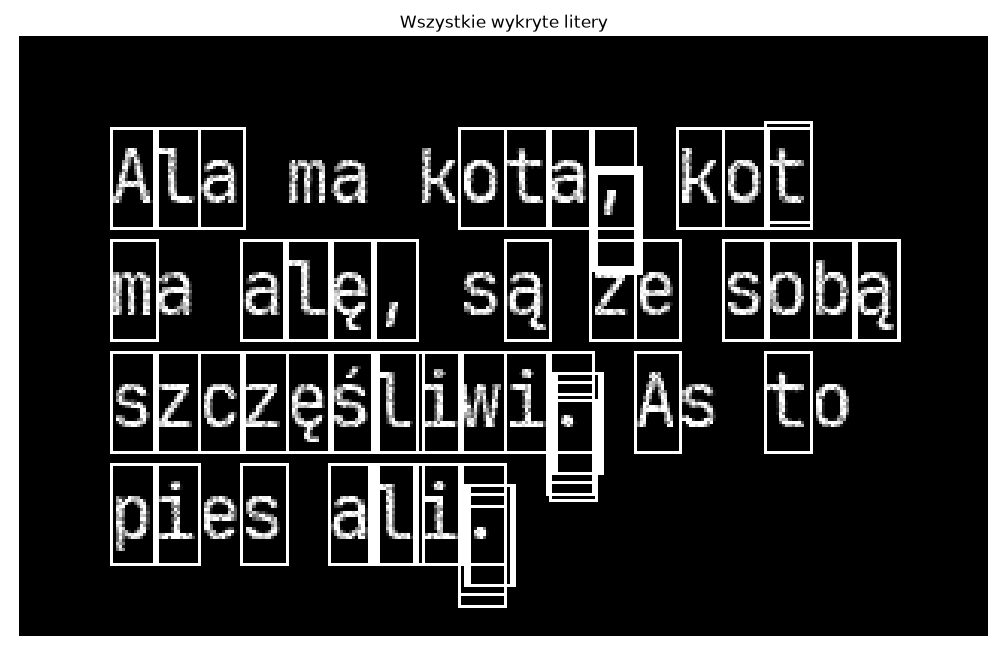
\includegraphics[width=\linewidth]{Obrazy/Korelacja/WykryteZnaki16.png}
  \caption{Wykryte znaki}
\end{figure}

Odtworzony tekst: Ala ota, kut m alę, ą ze subą szczęśliwi. A t p1 s ali. \\
Skuteczność: 15\% \\
Ocena czytelności: Nie wszystkie znaki zostały rozpoznane poprawnie, jednak sporą część sensu tekstu można zrozumieć.

\clearpage

\subsubsection{Szum Poissona dla $\lambda = 4$}

\begin{figure}[ht]
  \centering
  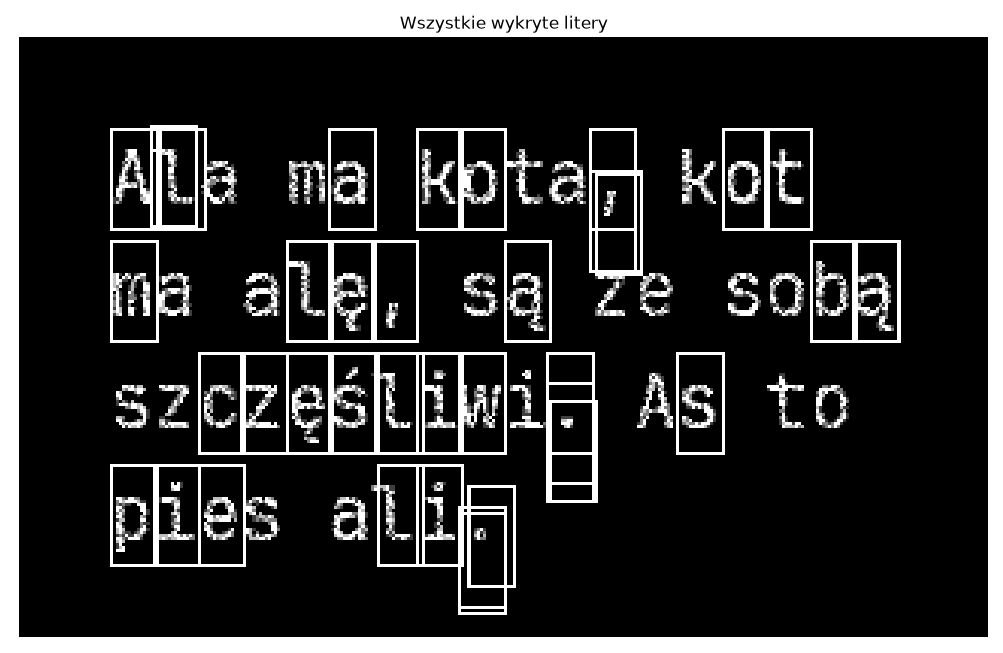
\includegraphics[width=\linewidth]{Obrazy/Korelacja/WykryteZnaki4.png}
  \caption{Wykryte znaki}
\end{figure}

Odtworzony tekst: AL a kn , ot m lę, ą ' bą częśLiw . s pie Li` \\
Skuteczność: 7\% \\
Ocena czytelności: Część znaków została rozpoznana prawidłowo. Nie można już odczytać sensu całego tekstu, natomiast można zrozumieć pojedyncze słowa.

\clearpage

\subsubsection{Szum Poissona dla $\lambda = 1$}

\begin{figure}[ht]
  \centering
  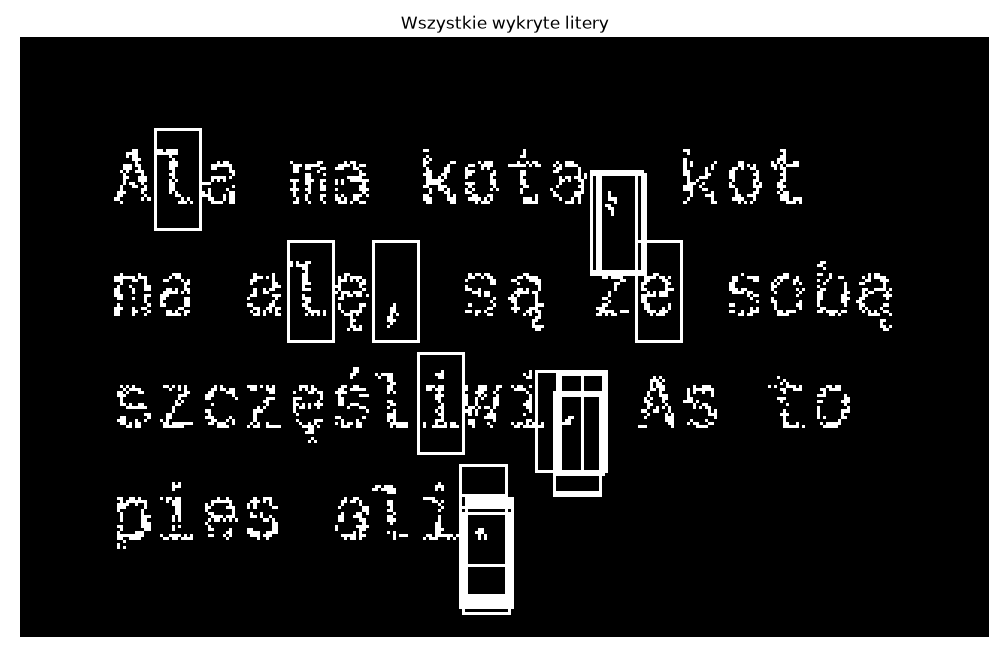
\includegraphics[width=\linewidth]{Obrazy/Korelacja/WykryteZnaki1.png}
  \caption{Wykryte znaki}
\end{figure}

Odtworzony tekst: l l , 'e i ~~ . \\
Skuteczność: 1\% \\
Ocena czytelności: Pojedyncze znaki zostały rozpoznane w większości prawidłowo. Zbyt mało znaków zostało rozpoznanych, aby odczytać sens tekstu.

\clearpage

\subsection{Rozpoznawanie tekstu za pomocą sieci neuronowej}
\subsubsection{Brak szumu Poissona}

\begin{figure}[ht]
  \centering
  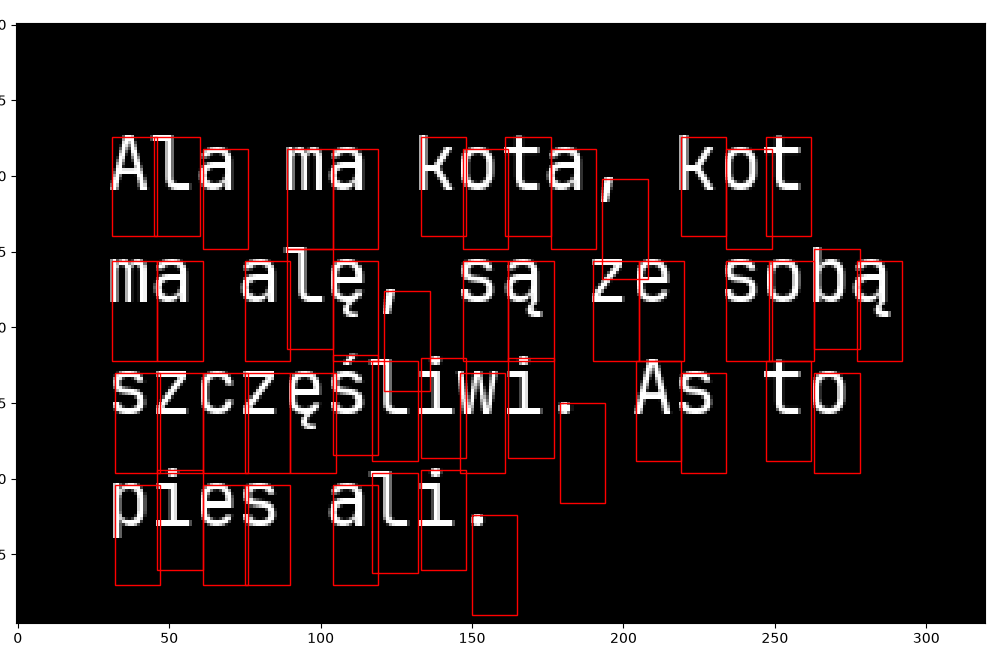
\includegraphics[width=\linewidth]{Obrazy/SiecNeuronowa/WykryteZnaki.png}
  \caption{Wykryte znaki}
\end{figure}

Odtworzony tekst: Ala ma kota, kot ma alę, są ze sobą szczęśliwi. As to pies ali. \\
Skuteczność: 100\% \\
Ocena czytelności: Odtworzony tekst jest identyczny z tekstu znajdującego się na obrazie wejściowym. Bez problemu można zrozumieć sens odtworzonego sensu.

\clearpage

\subsubsection{Szum Poissona dla $\lambda = 16$}

\begin{figure}[ht]
  \centering
  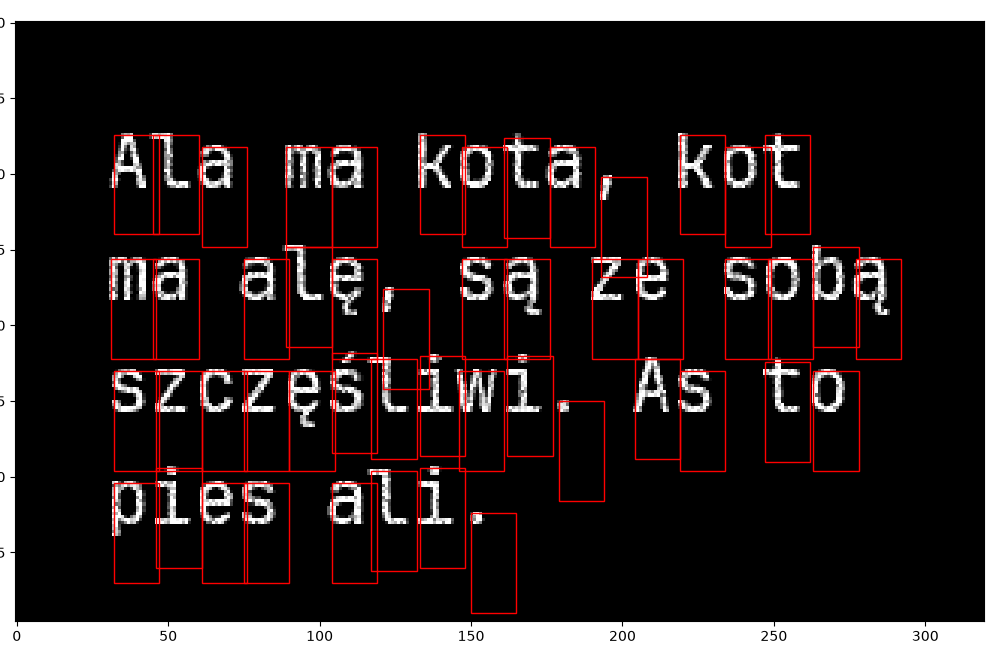
\includegraphics[width=\linewidth]{Obrazy/SiecNeuronowa/WykryteZnaki16.png}
  \caption{Wykryte znaki}
\end{figure}

Odtworzony tekst: Ala ma kota, kot ma alę, są ze sobą szczęśliwi. As to pies ali. \\
Skuteczność: 100\% \\
Ocena czytelności: Odtworzony tekst jest identyczny z tekstu znajdującego się na obrazie wejściowym. Bez problemu można zrozumieć sens odtworzonego sensu.

\clearpage

\subsubsection{Szum Poissona dla $\lambda = 4$}

\begin{figure}[ht]
  \centering
  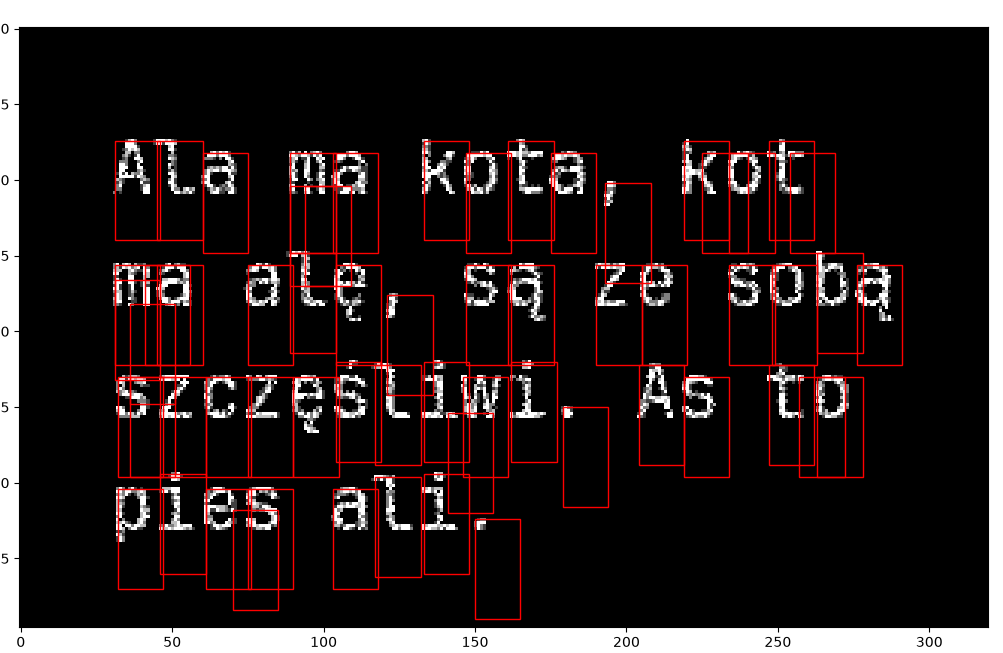
\includegraphics[width=\linewidth]{Obrazy/SiecNeuronowa/WykryteZnaki4.png}
  \caption{Wykryte znaki}
\end{figure}

Odtworzony tekst: Ala m..a koęa, K.ot. s,.!a alę, 9ą ze sobą s.zczęślj.wi. As t.o pie.s ali. \\
Skuteczność: 7\% \\
Ocena czytelności: Tekst został odtworzony w większości prawidłowo, jednak między prawidłowymi znakami zostały dodane znaki, których w oryginalnym tekście nie było. Mimo dodanych znaków tekst jest na tyle podobny do oryginału, że można wywnioskować z niego sens całego tekstu.


\clearpage

\subsubsection{Szum Poissona dla $\lambda = 1$}

\begin{figure}[ht]
  \centering
  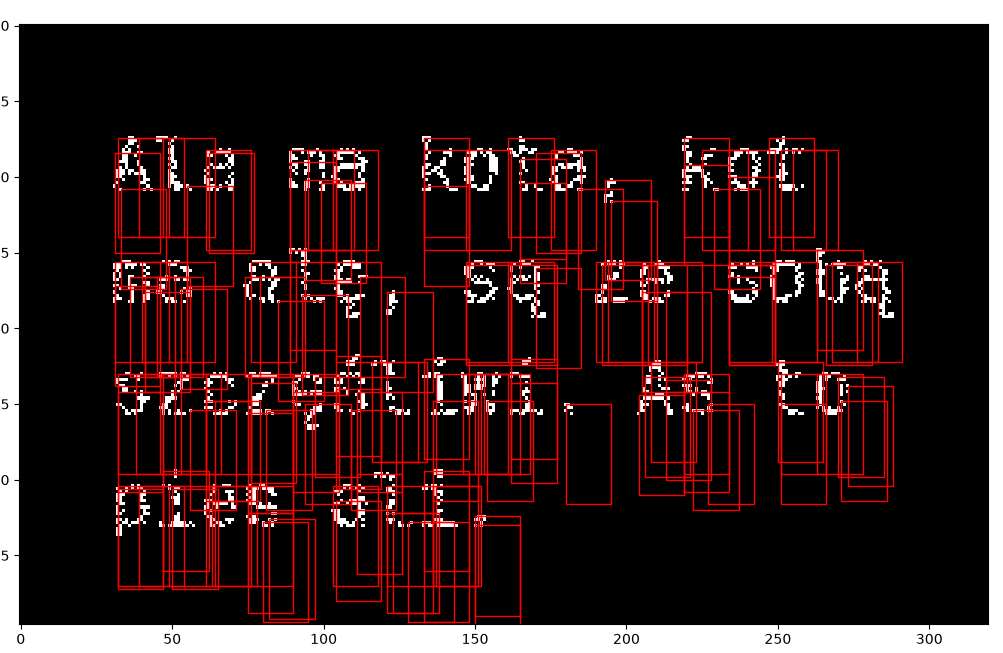
\includegraphics[width=\linewidth]{Obrazy/SiecNeuronowa/WykryteZnaki1.png}
  \caption{Wykryte znaki}
\end{figure}

Odtworzony tekst: \verb|HA.~l.aa ,x.*.a ,K.oo..Ja.,. kr..o~tI: o.,~~.s~. ,a:.1~ę., &są.,Zż,u~s. n,so| \\
\verb|!?.ą ,v.;:.r~ó~.,.s~,nxr..:ló~!*rs.*s. n,h~~a.. ,r~6... p,V.L.ese~.. ee^,.~.*.\t..| \\
Skuteczność: 3\% \\
Ocena czytelności: Część znaków została wykryta prawidłowo, jednak sporo znaków zostało wykryte błędnie i ponownie wiele znaków zostało dodane. Bardzo trudno wywnioskować sens oryginalnego tekstu.

\clearpage

\section{Analiza wyników}
\subsection{Rozpoznawanie tekstu za pomocą splotu}
W zastosowanej implementacji splot nie zapewnił poprawnego rozpoznawania tekstu. Wynika to z tego, że fragment obrazu (sygnału) wejściowego jest indeksowany inaczej niż filtr, z którym jest porównywany. Jeżeli filtr nie jest symetryczny, splot nie będzie w stanie znaleźć odpowiedniego dopasowania bez dodatkowego przekształcania obrazu (sygnału) wejściowego.

\subsection{Rozpoznawanie tekstu za pomocą korelacji wzajemnej}
Korelacja wzajemna dobrze rozpoznaje tekst z niezaszumionego obrazu. Niestety zaszumienie lub zniekształcenie obrazu (sygnału) wejściowego drastycznie zmniejsza skuteczność.

\subsection{Rozpoznawanie tekstu za pomocą sieci neuronowej}
Sieć neuronowa bardzo dobrze radzi sobie z rozpoznawaniem tekstu na obrazie. Nawet na silnie zaszumionym obrazie mogła rozpoznać niektóre znaki prawidłowo. Dodawanie znaków przez sieć wynika z metody przygotowania danych dla sieci. Algorytm szuka jednolitych fragmentów białego koloru i następnie przekazuje te fragmenty do sieci neuronowej. Przy silnym zaszumieniu obrazu znaki tracą swoją jednolitość i stają się kilkoma osobnymi fragmentami, z których sieć nie potrafi rozpoznać prawidłowego znaku. Dodatkowo skuteczność można poprawić ulepszając zbiór treningowy i trenując sieć dłużej. Ta metoda działa również dla różnych krojów czcionki i po odpowiednim treningu poradzi sobie nawet z rozpoznawaniem pisma odręcznego.

\section{Wnioski}
Po zbadaniu wykorzystania splotu i korelacji wzajemnej do rozpoznawania tekstu na obrazach rastrowych można stwierdzić, że splot nie nadaje się do rozpoznawania tekstu, natomiast można go zastosować do rozpoznawania innych prostszych elementów na obrazie. Natomiast korelacja wzajemna umożliwia prawidłowe odtworzenie tekstu o ile obraz wejściowy nie jest mocno zaszumiony bądź zniekształcony.

Z badań wykorzystania sieci neuronowej do rozpoznawania tekstu na obrazach rastrowych zauważyć można, że metoda ta jest skuteczniejsza niż splot oraz korelacja wzajemna. Mimo zaszumienia obrazu wejściowego, sieć neuronowa jest w stanie rozpoznać prawidłowo większość znaków, z których można wywnioskować sens tekstu znajdującego się na obrazie. Dodatkowo dopracowując metodę przetwarzania danych trafiających do sieci neuronowej można poprawić wyniki, a rozbudowując zbiór treningowy oraz wydłużając proces nauki modelu można z taką samą skutecznością rozpoznawać różne kroje czcionki, a nawet pismo odręczne.

\end{document}